\documentclass[12pt]{report}
% \documentclass[a4paper,9pt]{report}
\usepackage{iitbtitle}
\usepackage{iitbdeclaration}
\usepackage{iitbapproval}
\usepackage{a4wide}
\usepackage{anysize}
\usepackage{iitbcs}
\usepackage{latexsym}
\usepackage{amssymb}

\usepackage{charter}

\usepackage[dvips]{graphicx}
\DeclareGraphicsExtensions{.png,.jpg}

% \usepackage{inconsolata}
\usepackage[cm-default]{fontspec}
\setmainfont[Mapping=tex-text]{Times New Roman}

\usepackage{titlesec}
\titleformat{\chapter}[display]
{\normalfont\huge\bfseries\centering}{\chaptertitlename\ \thechapter}{18pt}{\Huge}

% \newcommand{\chapter}[1]{\chapter[#1]{\centering #1}} % this fails to center the chapter numbers as well!

% according to the guidelines, line spacing should be 1.5
\linespread{1.5}

% instead of Chapter 1, write only 1
\renewcommand{\chaptername}{}

\usepackage{geometry}

\geometry{
 a4paper,
 total={210mm,297mm},
 top=15mm,
 left=20mm,
 right=20mm,
 bottom=22mm,
 headsep=12mm,
 headheight=3mm,
 % footer=3mm,
 % footsep=10mm,
}

\usepackage[normalem]{ulem}
\usepackage[hidelinks,backref]{hyperref} % clickable links and citations with no green borders
\usepackage{amsmath}
\usepackage{listings} % add source code snippets
\usepackage{csquotes} % block quotes
\usepackage{color}
\usepackage{caption}
\usepackage{float}
\usepackage{subcaption}

% the bibliography should appear in the table of contents
\usepackage[nottoc]{tocbibind}

% reduce table of contents spacing
\usepackage[titles]{tocloft}
\setlength{\cftbeforechapskip}{.1ex}
\setlength{\cftbeforesecskip}{-.5ex}

\setlength{\parindent}{12mm} % paragraph indentation
\setlength{\parskip}{3mm} % paragraph spacing

\marginsize{2.5cm}{2.5cm}{1cm}{1.5cm}
\def\baselinestretch{1.15}                          

\newcommand\INPUT{\item[\textbf{Input:}]}
\newcommand\OUTPUT{\item[\textbf{Output:}]}

% define some colors
\definecolor{mygreen}{rgb}{0,0.6,0}
\definecolor{mygray}{rgb}{0.5,0.5,0.5}
\definecolor{mydarkgray}{rgb}{0.4,0.4,0.4}
\definecolor{mymauve}{rgb}{0.58,0,0.82}
\definecolor{myrust}{rgb}{0.77,0,0}
\pagestyle{empty}

\lstset{ %
  backgroundcolor=\color{white},   % choose the background color; you must add \usepackage{color} or \usepackage{xcolor}
  basicstyle=\footnotesize\ttfamily,        % the size of the fonts that are used for the code
  breakatwhitespace=false,         % sets if automatic breaks should only happen at whiterspace
  breaklines=true,                 % sets automatic line breaking
  captionpos=b,                    % sets the caption-position to bottom
  commentstyle=\color{mygreen},    % comment style
  deletekeywords={...},            % if you want to delete keywords from the given language
  escapeinside={\%*}{*)},          % if you want to add LaTeX within your code
  extendedchars=true,              % lets you use non-ASCII characters; for 8-bits encodings only, does not work with UTF-8
  frame=single,                    % adds a frame around the code
  keepspaces=true,                 % keeps spaces in text, useful for keeping indentation of code (possibly needs columns=flexible)
  keywordstyle=\color{blue},       % keyword style
  language=C++,                    % the language of the code
  morekeywords={*,...},            % if you want to add more keywords to the set
  numbers=none,                    % where to put the line-numbers; possible values are (none, left, right)
  numbersep=5pt,                   % how far the line-numbers are from the code
  numberstyle=\tiny\color{mygray}, % the style that is used for the line-numbers
  rulecolor=\color{black},         % if not set, the frame-color may be changed on line-breaks within not-black text (e.g. comments (green here))
  showspaces=false,                % show spaces everywhere adding particular underscores; it overrides 'showstringspaces'
  showstringspaces=false,          % underline spaces within strings only
  showtabs=false,                  % show tabs within strings adding particular underscores
  stepnumber=2,                    % the step between two line-numbers. If it's 1, each line will be numbered
  stringstyle=\color{mymauve},     % string literal style
  tabsize=2,                       % sets default tabsize to 2 spaces
  % title=\lstname                   % show the filename of files included with \lstinputlisting; also try caption instead of title
}

\hypersetup{
  colorlinks=true,
  linkcolor=red,
  urlcolor=blue,
  citecolor=myrust,
  linktoc=page
}

\begin{document}

%\baselineskip 20pt
%The definitions
\def\title{A Generalized Model for Physically Simulating Burning}
\def\what{B. Tech. Stage I Project Report}
\def\degree{Bachelor~of~Technology}
\def\who{Rohan Prinja}
\def\roll{110050011}
\def\guide{Dr. Parag Chaudhuri}

\titlpage
\def\bsq{\begin{flushright} $\blacksquare$\\ \end{flushright}}
\def\tab{\hspace{5mm}}

\approvalpage
\declarationpage

%The stuff
\pagenumbering{roman}
\begingroup\def\thispagestyle#1{}\def\baselinestretch{1.5}\tableofcontents\endgroup     
\newpage
\begin{abstract}
Certain physical phenomena are too complicated to either model heuristically or be animated manually. By using the laws of physics we can develop realistic-looking animations. Our aim in this paper is to develop a generalized model for physically simulating burning that can be applied to a variety of objects, from thin-shell objects like paper to complicated volumetric objects like the Stanford bunny. Our model should be feature complete i.e. it should model all the phenomena associated with burning, like mass loss, smoke emission, object deformation and so on. Research on simulating burning of objects already exists, but it deals only with a subset of these features - for example, burning without deformation, flame simulation without burning, deformation only for thin-shell objects, and so on. There is a need for a generalized model that can handle all these cases together.

Following prior research, we implement fire as a coupled system of gases separated by an implicit surface. Smoke is treated as the gaseous product having cooled below a certain threshold. Objects are modeled as either triangular or tetrahedral meshes. We propose to handle mass loss by removing vertices from the mesh, and deformation by a change in the position of a vertex in the mesh relative to its neighbours.

We are currently implementing the flame simulation in two dimensions, and in the second phase of this project hope to complete the remainder of the tasks outlined above.
\end{abstract}
% %!TEX root = ./main.tex

% This file is part of the i10 thesis template developed and used by the
% Media Computing Group at RWTH Aachen University.
% The current version of this template can be obtained at
% <http://www.media.informatik.rwth-aachen.de/karrer.html>.

\loadgeometry{myAbstract}

\chapter*{Abstract\markboth{Abstract}{Abstract}}
\addcontentsline{toc}{chapter}{\protect\numberline{}Abstract}
\label{abstract}

%here (english version)
Lorem ipsum dolor sit amet, consectetur adipisicing elit, sed do eiusmod tempor incididunt ut labore et dolore magna aliqua. Ut enim ad minim veniam, quis nostrud exercitation ullamco laboris nisi ut aliquip ex ea commodo consequat. Duis aute irure dolor in reprehenderit in voluptate velit esse cillum dolore eu fugiat nulla pariatur. Excepteur sint occaecat cupidatat non proident, sunt in culpa qui officia deserunt mollit anim id est laborum.Lorem ipsum dolor sit amet, consectetur adipisicing elit, sed do eiusmod tempor incididunt ut labore et dolore magna aliqua. Ut enim ad minim veniam, quis nostrud exercitation ullamco laboris nisi ut aliquip ex ea commodo consequat. Duis aute irure dolor in reprehenderit in voluptate velit esse cillum dolore eu fugiat nulla pariatur. Excepteur sint occaecat cupidatat non proident, sunt in culpa qui officia deserunt mollit anim id est laborum.Lorem ipsum dolor sit amet, consectetur adipisicing elit, sed do eiusmod tempor incididunt ut labore et dolore magna aliqua. Ut enim ad minim veniam, quis nostrud exercitation ullamco laboris nisi ut aliquip ex ea commodo consequat. Duis aute irure dolor in reprehenderit in voluptate velit esse cillum dolore eu fugiat nulla pariatur. Excepteur sint occaecat cupidatat non proident, sunt in culpa qui officia deserunt mollit anim id est laborum.Lorem ipsum dolor sit amet, consectetur adipisicing elit, sed do eiusmod tempor incididunt ut labore et dolore magna aliqua. Ut enim ad minim veniam, quis nostrud exercitation ullamco laboris nisi ut aliquip ex ea commodo consequat. Duis aute irure dolor in reprehenderit in voluptate velit esse cillum dolore eu fugiat nulla pariatur. Excepteur sint occaecat cupidatat non proident, sunt in culpa qui officia deserunt mollit anim id est laborum.

\chapter*{\"Uberblick\markboth{\"Uberblick}{\"Uberblick}}
\addcontentsline{toc}{chapter}{\protect\numberline{}\"Uberblick}
\label{ueberblick}

%here (deutsche version)
Lorem ipsum dolor sit amet, consectetur adipisicing elit, sed do eiusmod tempor incididunt ut labore et dolore magna aliqua. Ut enim ad minim veniam, quis nostrud exercitation ullamco laboris nisi ut aliquip ex ea commodo consequat. Duis aute irure dolor in reprehenderit in voluptate velit esse cillum dolore eu fugiat nulla pariatur. Excepteur sint occaecat cupidatat non proident, sunt in culpa qui officia deserunt mollit anim id est laborum.Lorem ipsum dolor sit amet, consectetur adipisicing elit, sed do eiusmod tempor incididunt ut labore et dolore magna aliqua. Ut enim ad minim veniam, quis nostrud exercitation ullamco laboris nisi ut aliquip ex ea commodo consequat. Duis aute irure dolor in reprehenderit in voluptate velit esse cillum dolore eu fugiat nulla pariatur. Excepteur sint occaecat cupidatat non proident, sunt in culpa qui officia deserunt mollit anim id est laborum.Lorem ipsum dolor sit amet, consectetur adipisicing elit, sed do eiusmod tempor incididunt ut labore et dolore magna aliqua. Ut enim ad minim veniam, quis nostrud exercitation ullamco laboris nisi ut aliquip ex ea commodo consequat. Duis aute irure dolor in reprehenderit in voluptate velit esse cillum dolore eu fugiat nulla pariatur. Excepteur sint occaecat cupidatat non proident, sunt in culpa qui officia deserunt mollit anim id est laborum.Lorem ipsum dolor sit amet, consectetur adipisicing elit, sed do eiusmod tempor incididunt ut labore et dolore magna aliqua. Ut enim ad minim veniam, quis nostrud exercitation ullamco laboris nisi ut aliquip ex ea commodo consequat. Duis aute irure dolor in reprehenderit in voluptate velit esse cillum dolore eu fugiat nulla pariatur. Excepteur sint occaecat cupidatat non proident, sunt in culpa qui officia deserunt mollit anim id est laborum.


\loadgeometry{myText}

\newpage
\pagenumbering{arabic}

\chapter{Introduction}

In this chapter, we introduce the problem we are trying to solve in more detail, and motivate the use of physically-based simulation. We then outline the structure of the rest of this report.

\section{Aim of this project} % (fold)

In this project we aim to develop a framework for simulating the burning of an arbitrarily-shaped object. The inputs to this program will be a 3D object (described as either a mesh of triangles or tetrahedra) with certain parameters, like calorific value, rate of flame propagation, and so on. Along with this, we will have a list of coordinates corresponding to points on the surface of the object which are on fire at time $t = 0$. The output of this program will be a series of frames which can be stitched together into an animation. The animation will depict the propagation of flame across the surface of the object (for thin-shell objects) or the body of the object (for volumetric objects). As the flame progresses, the object will heat up and then burn, in the process deforming and losing mass. The object may burn directly or first melt and then burn (this is parametrizable). Burning byproducts like ash and smoke will be emitted.

\section{Why Use Physically-based Animation?} % (fold)
\label{sec:phys_based_animation}

This project is about using physically-based methods to achieve photorealism in the context of simulating the behaviour of fire and its interaction with arbitrary objects in three dimensions. Photorealism in the context of computer graphics means creating renderings or animations that look as similar to real life as possible.

Simulating fire is an instance of a more general problem - we have materials which are known to follow some physical laws and we want to animate them over some time frame. The hard part is doing this realistically. Physically-based simulation is a way to do so. Before physical simulation was a viable option, photorealism in simulating materials was traditionally achieved in one of two ways:

\begin{enumerate}
  \item Skilled animators, designers and artists would manually draw or adjust each frame of the animation in order to make it look real. The obvious problem with this approach is that it is slow. A 120-minute with 24 frames per second has 1,72,800 frames! A lot of manpower and time is needed if we want to make an animation longer than just a few minutes. Some amount of automation is necessary.
  \item We can model the materials to be animated by simple heuristics whose parameters can be tweaked to give the illusion of realistic behaviour. Flames, for example, can be simulated by Perlin noise, a relatively simple catch-all model (used in many diverse areas) that does not take into account any of the physical properties of fire. Although this is in practice very easy to implement, there are two problems with this approach.
  \begin{enumerate}
    \item A large amount of tweaking is required to get the heuristics just right, and in any case, we are not really simulating the behaviour of the material as much as simply using ``hacks" to get the job done. This limits the extent to which our results can be photorealistic.
    \item Another problem is that in the real world, interactions between objects can become quite complicated. When a white sheet of paper is burnt, fire propagates across the sheet. The paper becomes discolored, going from white to brown and then black. The paper deforms at the point of burning, and this burning is often directly proportional to the strength of the flame at that point. The deformation itself affects the precise way in which the flame will spread from the currently burning portion to the rest of the paper. Little bits of ash may fall off as the burning progresses. Smoke is emitted by the flame. A heuristic model to account for all these complex interactions would be complicated and unwieldy. Our only option then is to sacrifice accuracy for simplicity of implementation.
  \end{enumerate}
\end{enumerate}

Given these disadvantages, why is it only recently that physically-based methods have become popular? The answer is that we do not have closed-form solutions for simulating many physical phenomena. Instead, we usually have a system of differential equations that are solved by numerical methods, which are often slow. This means that computing the scene description of even a single frame of an animation on a personal computer can take a large amount of time, perhaps as many as a few seconds to a few minutes or more. Until recently, the hardware to efficiently process these computations had not yet caught up with software demands. Today, however, with the advent of more powerful methods of computation (parallel programming, GPUs, render farms, etc.) running time is no longer as big a barrier, and it is easier to achieve realism via physically-based animation.

\section{Difference from heuristic methods}

Like the heuristic methods described in \ref{sec:phys_based_animation}, we are using parameters to differentiate the behaviour of one type of object from another. However, the difference here is that we are the parameterization corresponds to actual physical properties of the object, for example, does the object melt or directly burn, what is the rate at which fuel escapes from the object surface and so on. In heuristic-based methods there may or may not be any direct relation between a simulation parameter and the physical properties of the materials involved in the simulation.

\section{Structure of this Report} % (fold)
\label{sec:structure_of_this_report}

In the following chapters of this report, we do a literature survey, then discuss the simulation of fire and smoke as an extension of the fluid simulation problem. We the look at how objects are modeled, and how possibly they can interact realistically with fire.

Now we look at the literature that is relevant to this project. We focus our attention on papers, theses and articles which have implemented some or most of the features involved in burning objects.

% section structure_of_this_report (end)

\chapter{Literature Survey}

In this chapter, we first discuss the features we would like to have in a unified model of burning objects, and discuss the literature on the implementation of these features.

\section{A Wishlist for a Unified Model of Burning} % (fold)
\label{sec:a_wishlist_for_a_unified_model_of_burning}

As mentioned above, a feature-complete burning simulation would include most or all of the following phenomena

\begin{enumerate}
  \item Flames and smoke. The flames spread across the surface of the object as the simulation progresses.
  \item Mass loss. The object should lose mass as the simulation progresses, since it is being converted to fuel which is used to feed the flame.
  \item The object might deform. By deformation we mean that certain parts of the object change the angles they make with other parts of the object. For example, if we burn the Stanford bunny, we might expect to see its ears droop. Or, as we burn a sheet of paper, it should crumple in on itself.
  \item Melting, possibly. An object need not necessarily burn directly, it may first melt and then the liquid will catch fire.
\end{enumerate}

All these phenomena have been well-studied. Below, we discuss some of these papers. However, there hasn't been much investigation into creating a model that unifies all of these features into a single simulation model. All of the following papers concentrate on implementing only a subset of these features, often with great results.

% section a_wishlist_for_a_unified_model_of_burning (end)

\section{Survey of previous work} % (fold)
\label{sec:survey_of_previous_work}

In \cite{festje}, the authors present a way to simulate smoke. This paper used a standard stable fluids approach as introduced in Stam's seminal paper \cite{stam}, and introduced vorticity confinement as a way to model the turbulence associated with smoke.

This paper was used in \cite{ngfeje}, in which the authors presented a framework for animating fire along with smoke. Flames are considered as the product of burning a gaseous fuel. The authors implement a coupled system consisting of two fluids - the fuel undergoing burning, and the hot gaseous product. A level-set is used to track the implicit surface that separates the fuel from the gaseous product. The paper also discusses burning of solid fuels. Points on the surface of the solid are assumed to be emitting gaseous fuel at a certain rate. In this way the solid burning case is reduced to the gas burning case. However, the paper is not concerned with the effects on the solid as the simulation progresses. Mass loss, deformation and residue formation are thus not dealt with, since the focus of the paper is rendering and animating flames.

In \cite{jiyoai}, the authors implement burning of the surface of volumetric objects. The main contribution of this project is a very fast GPU-based implementation of surface burning. However, flames are not simulated, and only mass loss is dealt with - object deformation is not modeled. Further more, the paper only deals with melting and not burning.

In \cite{liliansu}, the authors describe a method to burn thin-shell rigid objects like paper. They depict flames, and also model the object's deformation and discoloration as it burns. However, the scope of the paper does not extend to volumetric objects, or smoke simulation.

\cite{loirgufe} is the most feature-complete of them all. It describes a refined meshing procedure for solids and demonstrates melting of solids into liquids and deformation of thin-shell objects. However, it does not demonstrate melting alongside burning or deformation of volumetric objects. Thus there is room for improvement here as well.

\cite{melek} discusses a unified model of burning that involves smoke emission, combustion, heat distribution, mass loss, deformation and residue formation. However, it is interactive and real-time, and thus less photorealistic than other burning simulation attempts.

An interesting paper \cite{stomahkin} implements heat transport and phase-change for solids turning into liquids using the Material Point Method. MPM became popular in the graphics community after the publication of \cite{snow}, which explained how snow was implemented realistically in the animated movie `Frozen'.

% section survery_of_previous_work (end)

Having discussed the literature on burning of objects, we now look at each of the aspects involved in burning individually. In the next section, we look at fluid simulation and how it can be applied to the problem of simulating flames.

\chapter{An Introduction to Fluid Simulation}

Flames in a burning model are simulated using fluid simulation techniques. In our implementation we follow the approach outlined by \cite{ngfeje}, in which fire is treated as a coupled system of two fluids. The first fluid is the fuel being burnt. The second is the gas emitted when the first is burnt. The two fluids are separated by a roughly conical surface called the blue core. The fluid being burnt is inside the cone. The coupling comes from the fact that the blue core has to, at every step of the simulation accurately represent the boundary between the two fluids. To do this a level-set technique is used, and the level-set values are periodically corrected to avoid numerical inaccuracies.

In this chapter, we discuss the general problem of fluid simulation, and then explain in detail how \cite{ngfeje} builds on top of fluid simulation to simulate fire. To understand fluid simulation, we must start with the Navier-Stokes equations.

\section{The Navier-Stokes equations}

There are many ways to simulate fluids. The literature in computer graphics usually focuses on incompressible fluids. The techniques relevant to us are those which simulate the Navier-Stokes equations, sometimes referred to as the Euler equations. These fundamental equations describe the behaviour of an incompressible fluid by imposing constraints on the velocity field of the fluid. They are:

\begin{equation}\label{eq:navier1}
\nabla \cdot \mathbf{u} = 0
\end{equation}
\begin{equation}\label{eq:navier2}
\dfrac{\partial{\mathbf{u}}}{\partial{t}} = -(\nabla \cdot \mathbf{u})\mathbf{u} - \dfrac{1}{\rho}\nabla p + \nu \nabla^2\mathbf{u} + \mathbf{F}
\end{equation}

Here, $\mathbf{u}$ is the fluid velocity, $t$ is time, $\rho$ is the fluid density (assumed uniform everywhere), $p$ is the pressure, $\nu$ is the viscosity of the fluid (also assumed constant), and $\mathbf{F}$ is the external force field on the fluid (gravity, buoyancy, wind, etc.).

Equation~\ref{eq:navier1} says that any point inside the fluid, the divergence of the velocity field is zero. This means that at any point inside the volume occupied by the fluid, mass is neither being accumulated nor lost. This is a consequence of the fact that we are dealing only with incompressible fluids.

Equation~\ref{eq:navier2} is Newton's second law in the context of a (not necessarily incompressible) fluid element, minus the mass term. It says that the change in the velocity field over time is due to four things.

\begin{enumerate}
  \item The first term is the convection term. The momentum of the fluid is advected (``carried along") by the velocity field.
  \item The second term is the pressure term. Pressure differences within the fluid create forces on a fluid element.
  \item The third term is the diffusion term. The Laplacian operator measures the extent to which the neighbouring fluid elements differ from the current fluid element. The greater the difference, the greater the force exerted on the current fluid element. The viscosity of the fluid ``damps" this force - the larger it is, the less likely the fluid element is to respond to a velocity difference between itself and its neighbours.
  \item The fourth term is an external force field. This varies depending on the fluid we are simulating. For water and other liquids, it is typically gravity, which is implemented as a constant downward force field. For the gaseous fuel and the hot gaseous product in the flame simulation, it is buoyancy which varies from fluid element to fluid element depending on the temperature.
\end{enumerate}

There is no closed-form solution for the Navier-Stokes equations yet. So we have to actually update the velocity field by manually calculating the appropriate gradients. We now describe, at a high-level, a way to solve these equations.

\section{Solving the Navier-Stokes equations}

In this section, we describe Stam's stable fluids method, since it is the one used by the paper on which our fire implentation is based. A fluid is continuous, but in practice we simulate it on a discrete grid called the \textbf{MAC grid} (marker-and-cell grid). Each cell has a pressure variable $p$ and a density variable $\rho$ defined at its center, and velocity components $u_x$, $u_y$ and $u_z$ defined at its centre. These values are updated in each simulation step. The main program looks like this:

\lstset{language=C++}
\begin{lstlisting}
void main()
{
  intializeGrid();
  while (true)
  {
    updateGrid();
    renderGrid();
  }
}
\end{lstlisting}

The high-level algorithm for updateGrid() for a semi-Lagrangian stable fluids update is:
\lstset{language=C++}
\begin{lstlisting}
void updateGrid()
{
  updateTemperature();
  addExternalForces(); //add gravity, buoyancy, etc. to each MAC cell
  advectVelocity(); //advect the velocity field along itself
  diffuseVelocity(); //spread the velocity field around to represent velocity
  projectAndPressureSolve(); //remove divergence created above (Navier-Stokes #1)
  // and also solve for pressure using a black-box linear-equation-system solver
}
\end{lstlisting}

The main contribution of Stam's stable fluids paper was that advection was done in a semi-implicit way. Previously, velocity was advected by taking velocities from adjacent grid cells. This led to unstable simulations which were controlled by carefully adjusting the timestep. Stam used the method of characteristics, which is unconditionally stable, that is, it is guaranteed not to become unstable for even large time steps. In the \texttt{advectVelocity()} step, to find the new velocity at a point $x$ (located at the center of a grid cell), we walk backwards along the velocity field \textbf{u} for time $\delta t$. Wherever we land, we obtain the new velocity by interpolating the current velocities. This new velocity is the velocity at point $x$ after time $\delta t$.

\section{Flame simulation using stable fluids}

\subsection{Extensions to Stam's paper}

In \cite{ngfeje}, the authors take the ideas presented in Stam's paper and apply it to the problem of simulating fire. In addition to the above-mentioned simulation variables, we also store the unit normal at each grid cell for which the level-set value is non-positive, that is, we store the unit normal at each point in the region occupied by the gaseous fuel as well as the implicit surface.

We also have two balance equations used to conserve mass and momentum across the implicit surface:

\begin{equation}
\rho_h(V_h - D) = \rho_f(Vf - D)
\end{equation}
\begin{equation}
\rho_h(V_h - D)^2 + p_h = \rho_f(Vf - D)^2 + p_f
\end{equation}

where $p_h$ and $p_f$ are the pressures of the hot gaseous products and the gaseous fuels, and $\rho_f$ and $\rho_f$ are the corresponding densities. Similarly, $V_h$ and $V_f$ are the components of the velocities of the gases in the normal direction (normal with respect to the implicit surface), and $D$ is the speed of the implicit surface in the normal direction. We have $D = V_f - S$, where $S$ is a fuel parameter proportional to the rate at which the fuel burns i.e. the rate at which the gaseous fuel is converted to the hot gaseous product.

The implicit surface itself is represented by a level-set defined at the centre of each grid cell, which is updated at each time step. We also store a scalar representing temperature at each grid cell. Every few time steps, numerical error will build up so a fast-march technique (see \cite{sethian}) is used to correct the level-set values.

\subsection{The ghost fluid method}

The other problem to take care of in a coupled system is that the advection step involves moving a particle `backwards' in time. For a particle in the gaseous product fluid, tracing backwards might take us to a position in the gaseous fuel region. We would then be interpolating velocities from one fluid to assign a new velocity for the other fluid, which is wrong. To solve this problem, the authors make use of the ghost fluid method introduced in \cite{ghost}. Say we are tracing back a fuel particle and we end up in the region occupied by the gaseous product. Instead of interpolating the gaseous product velocities we interpolate the ghost fluid velocities, where the ghost fluid velocity is given by

\begin{equation}
\mathbf{u}^G_h = V^G_h\mathbf{n} + \mathbf{u}_f - (\mathbf{u}_f\cdot\mathbf{n})\mathbf{n}
\end{equation}

Here, $V_f$ is the normal velocity of the fuel computed as $V_f = \mathbf{u}_f\cdot\mathbf{n}$, where $\mathbf{n}$ is the unit normal. The velocity $V^G_h$ is computed as

\begin{equation}
V^G_h = V_f + (\dfrac{\rho_f}{\rho_h} - 1)S
\end{equation}

How do we know when we have crossed the implicit surface and are now in a different region than the one we started in? We simply check if the sign of the level-set function has changed while crossing over or not.

\subsection{Evolving temperature and density}

For temperature, we evolve a scalar variable Y which takes values in the range $[0, 1]$. This variable is then mapped to the temperature using a temperature curve identified by the authors. The temperature curve as show in figure~\ref{fig:tempcurve} describes the rise and fall of the temperature of a gaseous fuel during the course of the burning. The authors also identify a computationally cheap alternative to mapping to the temperature falloff region of the curve (in which the temperature has reached its peak value and now only decreases).

\begin{figure}[H]
\centering
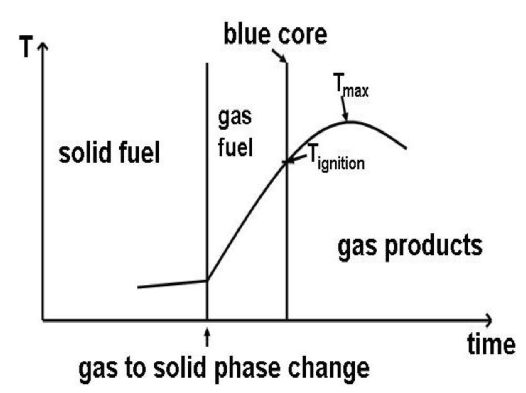
\includegraphics[width=.5\linewidth]{img/temperature}
\caption{Flame temperature profile for a fuel (courtesy \cite{ngfeje})}
\label{fig:tempcurve}
\end{figure}

For smoke, we evolve a scalar variable representing density. When the value of this variable falls below a certain threshold, smoke is seen. The authors also propose simulating soot by adding particles to the smoke.

Having looked at the stable fluids method in the context of fire and smoke simulation, we now turn our attention to how to model the objects being burnt.

\chapter{Modeling Objects}

In this section we discuss how to model objects on which burning is being simulated. We classify objects as 2D or 3D, and if 3D, as thin-shell or volumetric. The solid is meshed appropriately. Our flame propagation algorithm operates on this mesh.

\section{Meshing 2D objects}

2D objects are simulated as a mesh of triangles. For this, the \textbf{Triangle} tool \cite{shewchuk} is used. When invoked from the command line with a \texttt{.poly} file as input, it generates the DeLaunay triangulation of the surface represented by that file and writes the result into a few related files.

\begin{figure}[H]
\centering
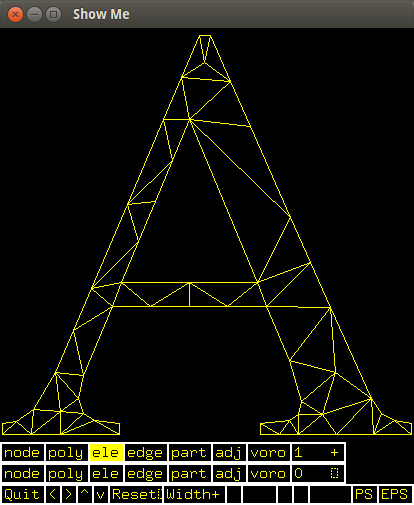
\includegraphics[width=.5\linewidth]{img/triangle}
\caption{Triangulating a 2D ``A" (UI courtesy the \texttt{triangle} base source code)}
\label{fig:atriangle}
\end{figure}

Figure~\ref{fig:atriangle} shows the result of invoking the \texttt{triangle} binary on a \texttt{.poly} file with the flags \texttt{-q} (quality triangulation) and \texttt{-a0.02} (maximum area constraint of 0.02).

\section{Meshing 3D objects}

We consider two kinds of 3D objects - \textbf{thin shell objects} and \textbf{volumetric objects}. Thin-shell objects have no thickness, for example, paper, cloth and hollow spheres. We only need to mesh the surfaces of such objects using triangles. Volumetric objects by contrast are solid. We model these objects as a mesh of tetrahedra. For this we use the \href{http://www.tetgen.org/}{\texttt{tetgen}} tool. Like \texttt{trigen}, it generates a DeLaunay tetrahedralization of a given volume. \texttt{tetgen} accepts various parameters which affect the process of tetrahedralization. For example, passing the \texttt{-a} option with a numerical argument $V$ when invoking \texttt{tetgen} ensures that limit the maximum volume over all tetrahedra in the output is $V$. Figure~\ref{fig:lmesh} is an example of tetrahedralizing a L-shaped volumetric block.

\begin{figure}[H]
\centering
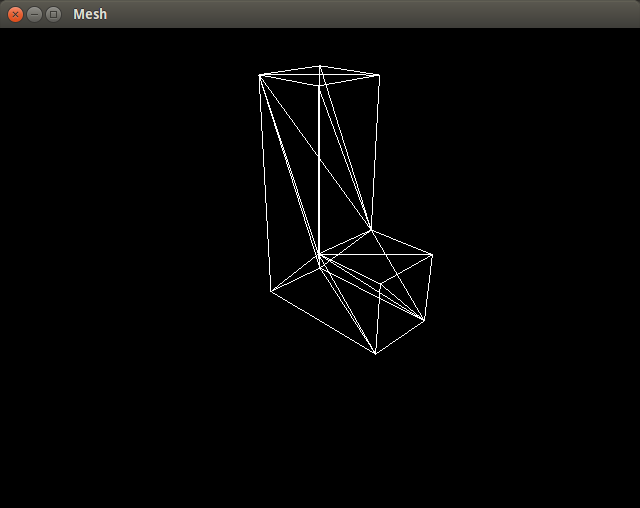
\includegraphics[width=\linewidth]{img/lmesh}
\caption{Meshing a 3D volumetric L block}
\label{fig:lmesh}
\end{figure}

\section{Input format}

\texttt{triangle} takes as input a file in the \texttt{.poly} format. It is a format for representing a Planar Straight Line Graph. Details of the \texttt{.poly} format can be found \href{http://www.cs.cmu.edu/~quake/triangle.poly.html}{here}.

\texttt{tetgen} takes as input a file in the \texttt{.smesh} format. \texttt{smesh} stands for surface mesh. It is a format for representing Piecewise Linear Complexes. Each facet of the input object is considered to be made up of one polygon. We assume no holes or points inside the object. When passed the \texttt{-k} flag, it outputs a \texttt{.vtk} file. The VTK format is a convenient way to store meshes. To visualize these meshes, we can use the \textbf{Paraview} mesh viewer and editor, or the VTK viewer we wrote.

Now that we have a way to mesh arbitrary objects, we look at how such meshes interact with flames.

\chapter{Interaction of object and fire}

In the preceding chapters we described how objects are modeled and how fire and smoke are simulated. Now we look at how objects react to being burnt. First we enumerate some phenomena that occur when an object is set on fire. Then we mention a novel technique that might be useful for this project.

\section{Phenomena associated with burning}

When an object is on fire, it heats up, and this heat is transported throughout the solid. Due to heat differences, the object may even deform. Since the solid is being burnt to provide fuel for the flame, it must also lose some of its mass. This means removal of vertices from the mesh. However, if we simply remove vertices from the mesh we end up with an incomplete or `broken' mesh. So re-meshing needs to be done whenever mass is lost from the mesh. \cite{loirgufe} describes a meshing technique which we could use.

\section{Material Point Method}

We have not yet settled on an exact framework for flame and heat propagation, but we are currently investigating using the Material Point Method as presented by \cite{stomahkin} in a recent paper.

\begin{figure}[H]
\centering
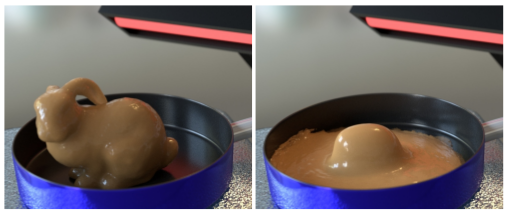
\includegraphics[width=\linewidth]{img/bunnymelt}
\caption{Melting a chocolate replica of the SIGGRAPH bunny (courtesy \cite{stomahkin})}
\label{fig:bunny_figure}
\end{figure}

As can be seen in figure~\ref{fig:bunny_figure}, the MPM simulates heat transport very well, allowing for realistic melting.

\chapter{Results and future work}

\section{Heuristic Burning}

We implemented a heuristic method for interactively burning a 2D object like paper as a proof-of-concept, and to demonstrate the infeasibility of heuristic-based methods. In this section we explain the algorithm and evaluate its behaviour.

\subsection{Overview}

We divide the surface of the object into square cells and probabilistically propagate a flame from a cell to its four neighbours. Initially some points are chosen as sources of burning. Once the \texttt{space} key is pressed the flame  propagates outwards from each burning source. We have no concept of temperature. Each cell on the object is in one of three states: \textit{unburnt}, \textit{burning} and \textit{burnt}. All cells are initially \textit{unburnt}. In each simulation step, every burning cell has a chance to spread the flame to each of its four neighbours with a certain probability (this is a parameter of the simulation). Once a cell enters the \textit{burning} state, it stays in that state for a fixed number of simulation steps (this is also a parameter), and then enters the \textit{burnt} state. For rendering, we color \textit{burning} cells depending on the amount of time they have remained in the burning state. \textit{burnt} cells are black.

Figure~\ref{fig:paperburn} shows two example runs of the problem, with different initial point sets.

\begin{figure}[H]
\centering
\begin{subfigure}{.48\textwidth}
  \centering
  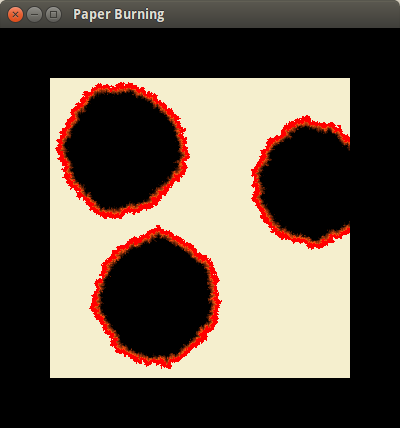
\includegraphics[width=\linewidth]{img/paper1}
  \caption{3 initial points in the interior}
\end{subfigure}
\begin{subfigure}{.48\textwidth}
  \centering
  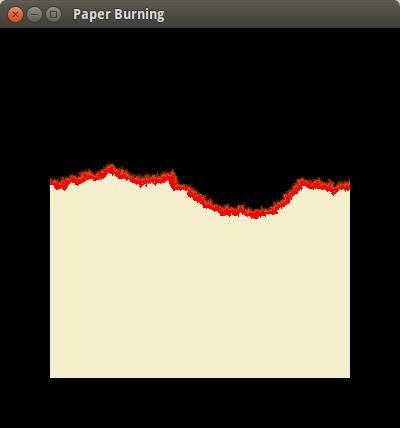
\includegraphics[width=\linewidth]{img/paper2}
  \caption{5 initial points near the top}
\end{subfigure}
\caption{A heuristic-based method for simulating paper burning}
\label{fig:paperburn}
\end{figure}

\subsection{Evaluation}

We observe that a lot of fine-tuning is needed to get a good simulation. The probability value needs to be set carefully. If it is too low, the flame dies out too quickly and ends up leaving a small circular hole roughly centred at the point where burning began. If it is two high, the flame begins to resemble an outward-growing rectangle, which looks completely unrealistic. Furthermore, deformation, actual flame simulation and smoke are not covered by this simplistic model. Photorealism is absent. This proof-of-concept program verifies the need for physically-based animation as an alternative to na\"ive heuristic-based methods that only approximate reality instead of describing it.

At the same time, there are some features of this model that we will use in our actual physically-based simulation, namely, propagating flame from nodes to neighbour nodes (except not probabilistically), and transitioning cells from unburnt to burning to the burnt state.

\section{Tetrahedral Meshing}

We implemented a class for representing tetrahedral meshes and integrated it into \textbf{Mantaflow}~\cite{mantaflow}, a fluid simulation framework. To test it out, we wrote a VTK visualizer which loads a \texttt{.vtk} file and parses it into a tetrahedral mesh object.

\section{Flame simulation}

Currently, we are implementing a 2D smoke-and-fire simulation based on \cite{ngfeje} in a framework forked from \cite{caltech}'s implementation for simulating a smoke plume, with some material taken from \cite{harsha}'s implementation for simulating water in 2D. Once this is complete, we will add interaction with triangulated 2D meshes to the extent that the flame treats the object just as an obstacle. After this, we plan to incorporate a flame-object interaction model, and then extend the program to 3D.

\chapter{Summary and Conclusions}

In conclusion, we have identified a need for a unified model satisfying the following:

\begin{enumerate}
  \item Simulations produced by it are realistic
  \item Simulates not just the flame but also smoke, soot and (possibly also) residue formation
  \item Applies to both thin-shell and volumetric objects
  \item Models object deformation and mass loss
\end{enumerate}

So far we have demonstrated the infeasibility of heuristic-based methods, shown meshing of arbitrary objects, begun work on the fire-and-smoke simulation and are trying to assess which model is best to model deformation and mass loss well.

\chapter{Acknowledgements}

I would like to thank my advisor, Prof. Parag Chaudhuri for providing advice and input on many aspects of the problem.

The code for the OpenGL VTK visualizer is a modified version of the code in \cite{dalling}. The modifications involved adding support for the \texttt{TetMesh} class.

For the fluid simulation framework, I originally used Mantaflow. Due to difficulties with the library, I abandoned it in favour of modifying \cite{caltech}'s source code for simulating smoke using Stam's stable fluids method. \cite{dmorris}'s explanation of the stable fluids paper was also invaluable.

\bibliography{report}{}
\bibliographystyle{alpha} % citations are numbered in order of appearance

\end{document}